\documentclass[12pt,executivepaper]{article}
\usepackage[utf8]{inputenc}
\usepackage[spanish]{babel}
\usepackage{amsmath}
\usepackage{amsfonts}
\usepackage{amssymb}
\usepackage{graphics}
\usepackage{graphicx}
\usepackage[left=1cm,right=1cm,top=2cm,bottom=2cm]{geometry}
\usepackage{imakeidx}
\makeindex[columns=3, title=Alphabetical Index, intoc]
\usepackage{listings}
\usepackage{xcolor}
\usepackage{multicol}
\usepackage{changepage}
\usepackage{float}
\usepackage{cite}
\usepackage{url}
\usepackage{hyperref}
\usepackage{pdfpages}

\definecolor{codegreen}{rgb}{0,0.6,0}
\definecolor{codegray}{rgb}{0.5,0.5,0.5}
\definecolor{codepurple}{rgb}{0.58,0,0.82}
\definecolor{backcolour}{rgb}{0.95,0.95,0.92}

\lstdefinestyle{mystyle}{
    backgroundcolor=\color{backcolour},
    commentstyle=\color{codegreen},
    keywordstyle=\color{magenta},
    numberstyle=\tiny\color{codegray},
    stringstyle=\color{codepurple},
    basicstyle=\ttfamily\footnotesize,
    breakatwhitespace=false,
    breaklines=true,
    captionpos=b,
    keepspaces=true,
    numbers=left,
    numbersep=5pt,
    showspaces=false,
    showstringspaces=false,
    showtabs=false,
    tabsize=3
}

\lstset{style=mystyle}
\author{González Pardo Adrian}
\date{Febrero 2020}

\title{Reporte de practica 2}
\newcommand\tab[1][1cm]{\hspace*{#1}}
\begin{document}
\maketitle
\section{Código VHDL}
\begin{center}
\lstinputlisting[language=VHDL]{./sources/sumador.vhd}
\textit{Código 1: Descripción del modulo sumador de 1 solo bit}
\end{center}
\begin{center}
\lstinputlisting[language=VHDL]{./sources/sumadorNBits.vhd}
\textit{Código 2: A través de uso de componentes de código para la descripción del sumador/restador en cascada de 8 bits}
\end{center}
\section{Test-Bench VHDL Código}
\begin{center}
    \lstinputlisting[language=VHDL]{./sources/simuSumador.vhd}
    \textit{Código de simulación}\\
    \textbf{Anexo de fotos de la simulación de impulsos}\\
\end{center}
\begin{flushleft}
	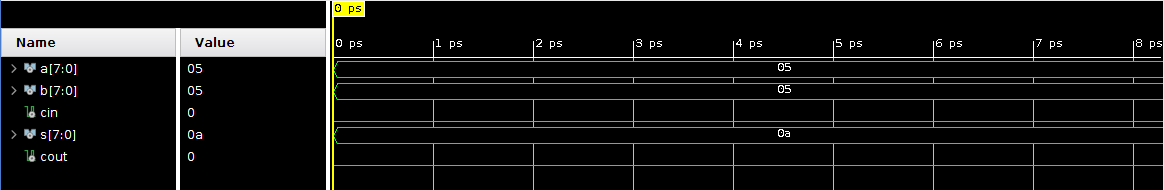
\includegraphics[scale=0.4]{imgs/primera.png}
\end{flushleft}
\begin{center}
    \textit{Primer parte con valores hexadecimales equivales a valores decimales: $a=5{\scriptscriptstyle10}$ $\&$ $b=5{\scriptscriptstyle10}$ con salida $s = A{\scriptscriptstyle16}= 10{\scriptscriptstyle10}$}
\end{center}

\begin{flushleft}
	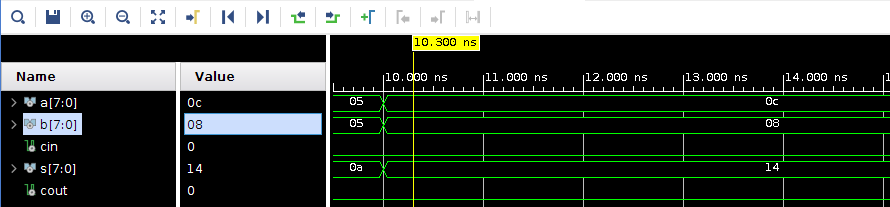
\includegraphics[scale=0.52]{imgs/segunda.png}
\end{flushleft}
\begin{center}
    \textit{Segunda parte con valores hexadecimales equivales a valores decimales: $a=C{\scriptscriptstyle16}=12{\scriptscriptstyle10}$ $\&$ $b=8{\scriptscriptstyle10}$ con salida $s = 14{\scriptscriptstyle16}= 20{\scriptscriptstyle10}$}
\end{center}

\begin{flushleft}
	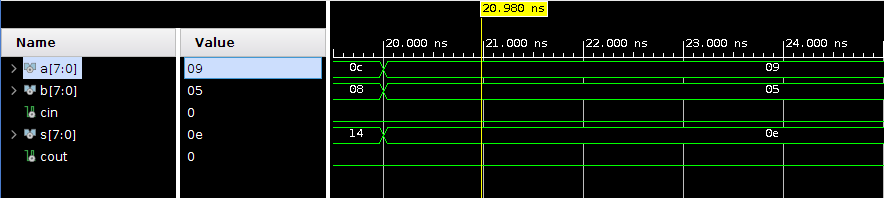
\includegraphics[scale=0.52]{imgs/tercera.png}
\end{flushleft}
\begin{center}
    \textit{Tercer parte con valores hexadecimales equivales a valores decimales: $a=9{\scriptscriptstyle10}$ $\&$ $b=5{\scriptscriptstyle10}$ con salida $s = E{\scriptscriptstyle16}= 14{\scriptscriptstyle10}$}
\end{center}


\begin{flushleft}
	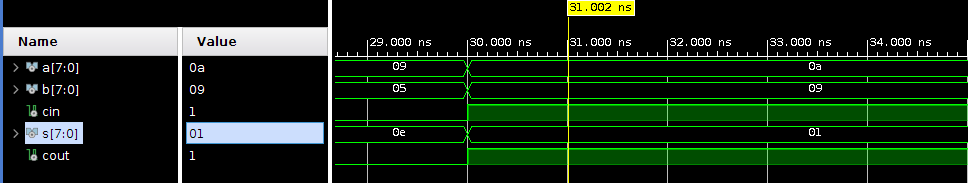
\includegraphics[scale=0.47]{imgs/cuarta.png}
\end{flushleft}
\begin{center}
    \textit{Cuarta parte con valores hexadecimales equivales a valores decimales: $a=A{\scriptscriptstyle16}=10{\scriptscriptstyle10}$ $,$ $b=9{\scriptscriptstyle10}$ $\&$ $cin=1{\scriptscriptstyle10}$ con salida $s =1{\scriptscriptstyle10}$ y un $cout=1{\scriptscriptstyle10}$}
\end{center}

\begin{flushleft}
	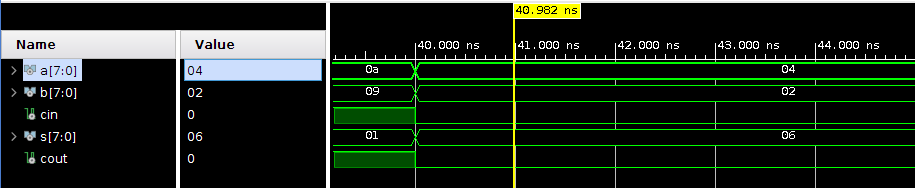
\includegraphics[scale=0.5]{imgs/quinta.png}
\end{flushleft}
\begin{center}
    \textit{Quinta parte con valores hexadecimales equivales a valores decimales: $a=4{\scriptscriptstyle10}$ $,$ $b=2{\scriptscriptstyle10}$ $\&$ $cin=0{\scriptscriptstyle10}$ con salida $s = 6{\scriptscriptstyle10}$}
\end{center}

\begin{flushleft}
	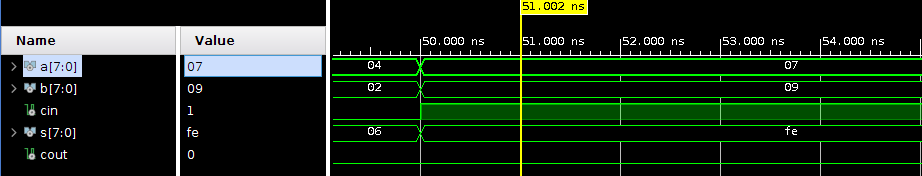
\includegraphics[scale=0.52]{imgs/sexta.png}
\end{flushleft}
\begin{center}
    \textit{Sexta parte con valores hexadecimales equivales a valores decimales: $a=7{\scriptscriptstyle10}$ $,$ $b=9{\scriptscriptstyle10}$ $\&$ $cin=1{\scriptscriptstyle10}$ con salida $s =FE{\scriptscriptstyle16}=254{\scriptscriptstyle10\_C2}=-2{\scriptscriptstyle10}$ y un $cout=0{\scriptscriptstyle10}$}
\end{center}

\begin{flushleft}
	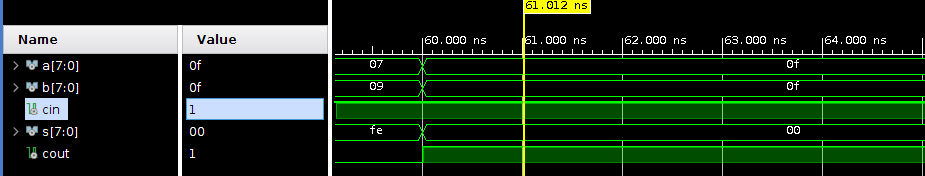
\includegraphics[scale=0.52]{imgs/septima.png}
\end{flushleft}
\begin{center}
    \textit{Septima parte con valores hexadecimales equivales a valores decimales: $a=F{\scriptscriptstyle16}=15{\scriptscriptstyle10}$ $,$ $b=F{\scriptscriptstyle16}=15{\scriptscriptstyle10}$ $\&$ $cin=1{\scriptscriptstyle10}$ con salida $s =0{\scriptscriptstyle10}$ y un $cout=1{\scriptscriptstyle10}$}
\end{center}

\begin{flushleft}
	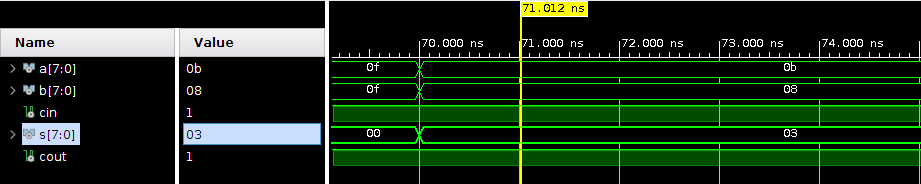
\includegraphics[scale=0.52]{imgs/octava.png}
\end{flushleft}
\begin{center}
    \textit{Octava parte con valores hexadecimales equivales a valores decimales: $a=B{\scriptscriptstyle16}=11{\scriptscriptstyle10}$ $,$ $b=8{\scriptscriptstyle10}$ $\&$ $cin=1{\scriptscriptstyle10}$ con salida $s =3{\scriptscriptstyle10}$ y un $cout=1{\scriptscriptstyle10}$}
\end{center}

\begin{flushleft}
	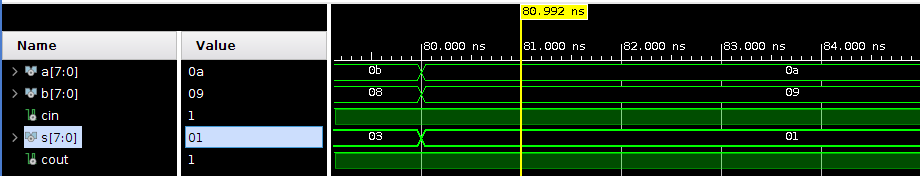
\includegraphics[scale=0.52]{imgs/novena.png}
\end{flushleft}
\begin{center}
    \textit{Novena parte con valores hexadecimales equivales a valores decimales: $a=A{\scriptscriptstyle16}=10{\scriptscriptstyle10}$ $,$ $b=9{\scriptscriptstyle10}$ $\&$ $cin=1{\scriptscriptstyle10}$ con salida $s =1{\scriptscriptstyle10}$ y un $cout=1{\scriptscriptstyle10}$}
\end{center}

\begin{flushleft}
	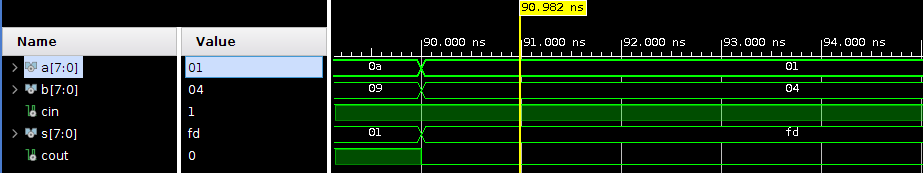
\includegraphics[scale=0.52]{imgs/decima.png}
\end{flushleft}
\begin{center}
    \textit{Decima parte con valores hexadecimales equivales a valores decimales: $a=1{\scriptscriptstyle10}$ $,$ $b=4{\scriptscriptstyle10}$ $\&$ $cin=1{\scriptscriptstyle10}$ con salida $s =FD{\scriptscriptstyle16}=253{\scriptscriptstyle10\_C2}=-3{\scriptscriptstyle10}$ y un $cout=0{\scriptscriptstyle10}$}
\end{center}
\section{Tabla de resultados}
\begin{center}
    \begin{tabular}{|p{2cm}|p{2cm}|p{2cm}|p{3cm}|p{2cm}|}
    \hline
    Operación & A & B & S & Cout \\\hline
    Suma & 5 & 5 & 10 & 0\\\hline
    Suma & 12 & 8 & 20 &0 \\\hline
    Suma & 9 & 5 & 14 & 0 \\\hline
    Resta & 10 & 9 & 1 & 1 \\\hline
    Suma & 4 & 2 & 6 & 0 \\\hline
    Resta & 7 & 9 & 254\_C2 = -2 & 0 \\\hline
    Resta & 15 & 15 & 0 & 1 \\\hline
    Resta & 11 & 8 & 3 & 1 \\\hline
    Resta & 10 & 9 & 1 & 1 \\\hline
    Resta & 1 & 4 & 253\_C2 = -3 & 0 \\\hline
    \end{tabular}
\end{center}
\clearpage
\section{Diagrama RTL}
\begin{center}
    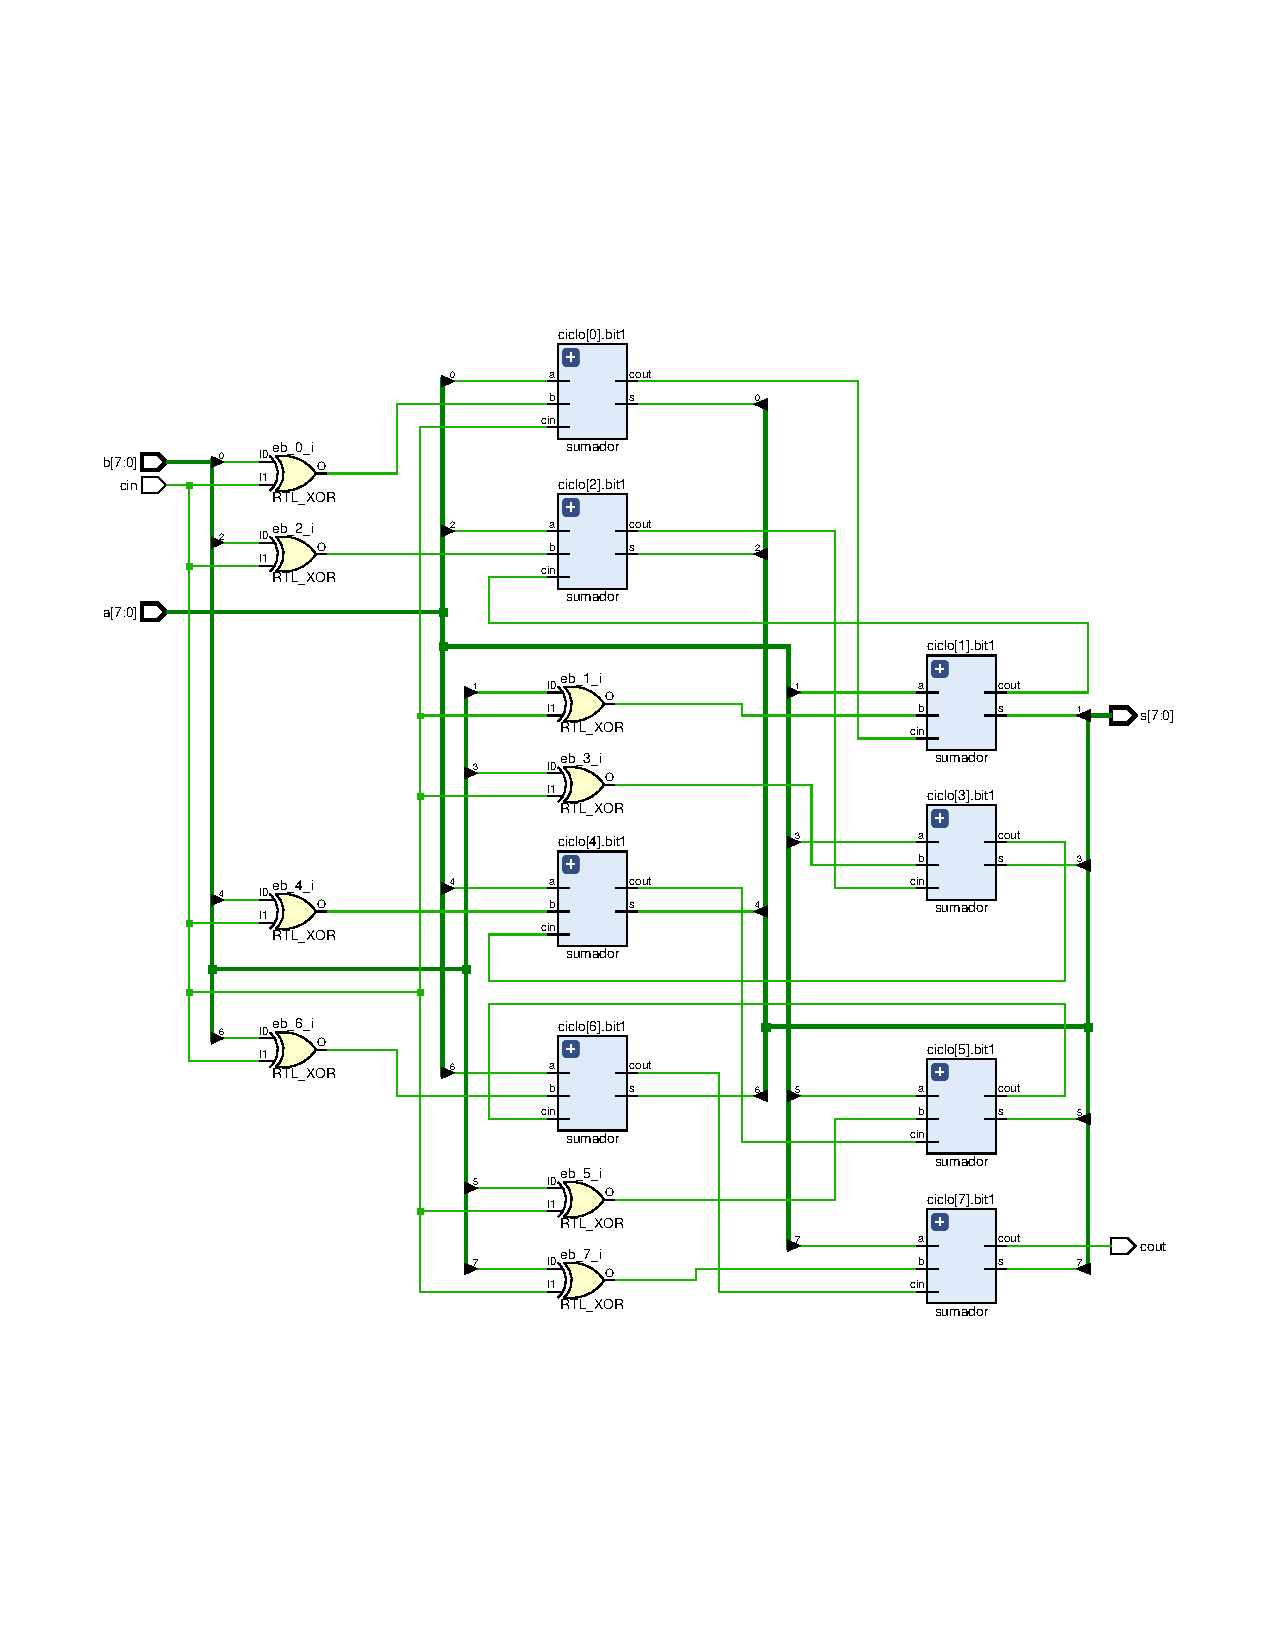
\includegraphics[scale=0.7]{sources/rtlDiagram.pdf}
    \textit{Diagrama RTL del archivo VHDL del sumador/restador en cascada de 8 bits}
\end{center}
\section{Diagrama de Síntesis}
\begin{center}
    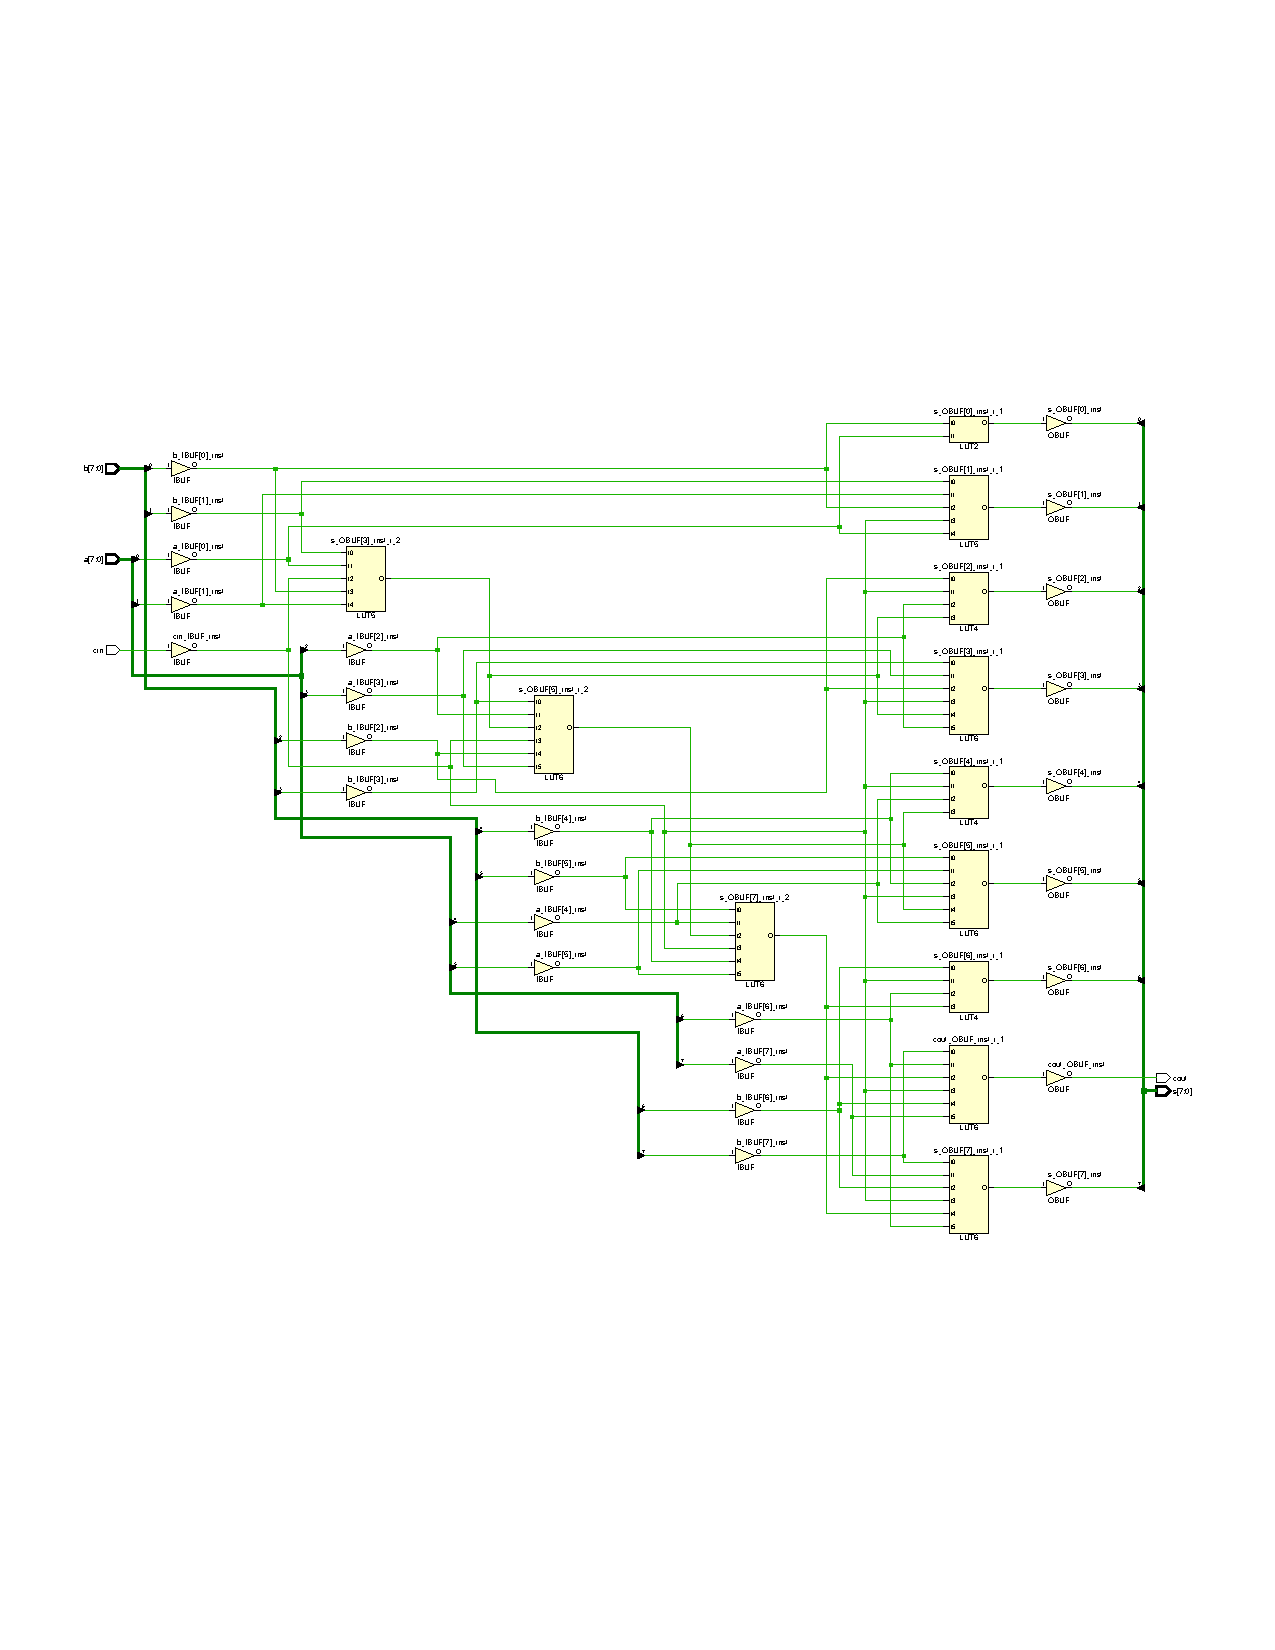
\includegraphics[scale=0.7]{sources/synthesisDiagram.pdf}
    \textit{Diagrama de Sintesis del archivo VHDL del sumador/restador en cascada de 8 bits}
\end{center}
\end{document}
